 \chapter{\label{chap:intro}Discussão}
 
%colocar em maiusculo tudo 
Na Figura a seguir (\ref{fig:cont1}) é possível observar os controles presentes na ISO 27002 que foram indicados pela maioria dos desenvolvedores de dispositivos móveis como os mais considerados quando elaboram uma aplicação. A seção da ISO que teve o maior numero de controles marcados como uma preocupação foi a seção de controle de acesso, seguido pelas seções de Aquisição, desenvolvimento e manutenção de sistemas, segurança nas operações e criptografia. As questões que tiveram respostas pouco expressivas ou neutras não foram consideradas na separação dos controles utilizados.

\begin{figure}[H]
\centering
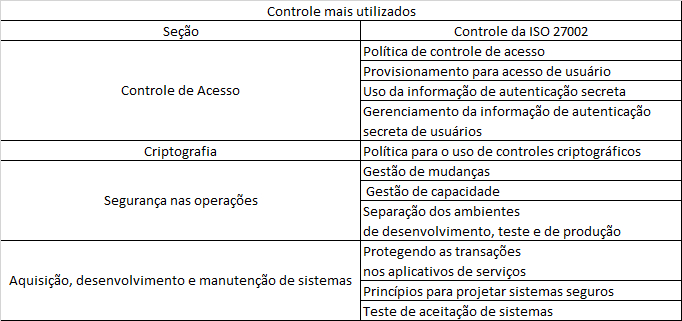
\includegraphics[scale=0.7]{fig2/maisusados.png}
\caption{Controles mais adotados pelos desenvolvedores}
\label{fig:cont1}
\end{figure}
%colocar em maiuculo

Na seção de controle de acesso quatro controles foram considerados como importantes pelos desenvolvedores, são eles:

\vspace{0.5cm}
\noindent\textbf{Política de controle de acesso:}
Todas as questões presentes neste controle que trata sobre a necessidade da implantação de um processo formal de registro e cancelamento de usuários, com o intuito de atribuir direitos de acesso foram considerados pelos desenvolvedores. 

\vspace{0.5cm}
\noindent\textbf{Provisionamento para acesso de usuário:}
Todas as questões presentes neste controle que trata sobre a implantação de um processo formal de provisionamentos de usuários para conceder e revogar direitos de acesso para todos os tipos de usuário em todos tipos de sistema foram considerados pelos desenvolvedores.

\vspace{0.5cm}
\noindent\textbf{Gerenciamento da informação de autenticação secreta de usuários:}
Duas das três questões selecionadas neste controle que trata sobre o controle do gerenciamento formal da  concessão de informação de autenticação secreta foram consideradas pelos desenvolvedores. A questão que não foi considerada pelos desenvolvedores, foi a questão Q2.2.

\vspace{0.5cm}
\noindent\textbf{Uso da informação de autenticação secreta:}
A questão presente neste controle que trata sobre a orientação que os usuários devem ter quanto a informação de autenticação secreta, foi considerada pelos desenvolvedores.

\vspace{0.5cm}

Na Seção de criptografia apenas um controle foi considerado pelos desenvolvedores como importante:

\vspace{0.5cm}
\noindent\textbf{Política para o uso de controles criptográficos:}
A questão presente neste controle, que trata sobre a implantação e desenvolvimento de uma política para o uso de controles criptográficos para proteção da informação, foi considerada importante pelos desenvolvedores.
\vspace{0.5cm}

Na seção sobre Segurança nas operações quatro controles foram considerados como importantes pelos desenvolvedores, são eles:

\vspace{0.5cm}
\noindent\textbf{Gestão de mudanças:}
A questão presente neste controle trata sobre a documentação e disponibilização dos procedimentos de operação para os usuários que necessitem, foi considerada pelos desenvolvedores.

\vspace{0.5cm}
\noindent\textbf{Gestão de capacidade:}
A questão presente neste controle trata sobre o monitoramento e utilização dos recursos para atender as necessidades de capacidade futura do sistema, foi considerada pelos desenvolvedores.

\vspace{0.5cm}
\noindent\textbf{Separação dos ambientes de desenvolvimento, teste e de produção:}
A questão presente neste controle que trata sobre a separação dos ambientes de desenvolvimento com o objetivo de reduzir os riscos de acessos ou modificações não autorizadas no ambiente de produção, foi considerada pelos desenvolvedores.

\vspace{0.5cm}
\noindent\textbf{Proteção das informações dos registros de eventos (logs):}
A questão presente neste controle trata sobre a proteção dos registros de eventos contra acesso não autorizado a adulteração, foi considerada pelos desenvolvedores.
\vspace{0.5cm}

Na seção sobre Aquisição, desenvolvimento e manutenção de sistemas três controles foram considerados pelos desenvolvedores, são eles:

\vspace{0.5cm}
\noindent\textbf{Protegendo as transações nos aplicativos de serviços}
 Todas as questões presentes neste controle, que trata sobre a proteção das transações em aplicativos de serviço, foram consideradas pelos desenvolvedores.

\vspace{0.5cm}
\noindent\textbf{Princípios para projetar sistemas seguros:}
Todas as questões presentes neste controle, que trata sobre necessidade princípios estabelecidos, documentados, mantidos e aplicados para a implantação de qualquer sistema de informação.

\vspace{0.5cm}
\noindent\textbf{Testes de aceitação de sistemas:}
Todas as questões presentes nesse controle, que trata sobre criação de testes de aceitação para novos sistemas,atualizações e novas versões, foram consideradas pelos desenvolvedores.

\vspace{0.5cm}

Na Figura \ref{fig:cont2} é possível observar os controles menos adotados pelos desenvolvedores de dispositivos móveis. A seção que possui os controles considerados menos relevantes é de controle de acesso, seguido pelas seções de segurança nas operações e Aquisição, desenvolvimento e manutenção de sistemas.

\begin{figure}[H]
\vspace{1cm}
\centering
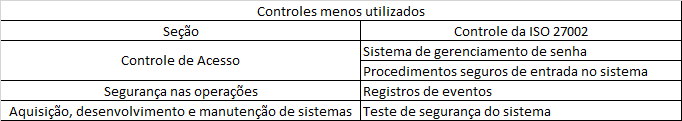
\includegraphics[scale=0.7]{fig2/menosusados.png}
\caption{Controles menos adotados pelos desenvolvedores}
\label{fig:cont2}
\end{figure}

\vspace{0.5cm}
\noindent\textbf{Sistema de gerenciamento de senha:}
Das três questões presentes no controle que trata de como assegurar senhas de qualidade, uma foi considerada relevante (Q2.13), outra inconclusiva (Q2.12) e a última não relevante (Q2.11).


\vspace{0.5cm}
\noindent\textbf{Procedimentos seguros de entrada no sistema (logon):}
Neste controle que trata sobre procedimentos seguros de entrada no sistema metade das questões foram consideradas relevantes (Q2.5, Q2.6 e Q2.7) e a outra metade ficou dividia entre duas questões inconclusivas (Q2.9 e 2.10) e uma não relevante (Q2.8).

\vspace{0.5cm}
\noindent\textbf{Registro de eventos:}
Neste controle que trata sobre produção e análise dos registro de eventos das atividades do usuário duas questões não foram consideradas relevantes (Q5.4 e Q5.5), uma foi inconclusiva (Q 5.3).

\vspace{3cm}
\noindent\textbf{Testes de segurança do sistema:}
 Neste controle que trata sobre a realização de testes de funcionalidade durante o desenvolvimento de sistemas de Uma das três questão foi considerada como não relevante (Q 6.14) pelos desenvolvedores.


A partir de resultado foi possível observar que muitos dos controles estavam sendo adotados pelos desenvolvedores. Uma hipótese para esse resultado é o fato de que 19 dos 20 respondentes trabalham em equipe e desenvolvem aplicações pra uso empresarial, o que pode indicar que os desenvolvedores seguem orientações ou práticas institucionalizadas nas organizações. Para identificar os motivos que levaram os desenvolvedores a considerarem os controles da ISO 27002 uma preocupação ou não, poderia-se realizar um estudo futuro, com uma nova entrevista com especialistas afim de identificar os possíveis motivos que levam os desenvolvedores a não darem tanta importância a esses cuidados.